\documentclass[conference]{IEEEtran}
\usepackage[utf8]{inputenc}
\usepackage[T1]{fontenc}
\usepackage{lmodern}
\usepackage[english]{babel}
\usepackage{amsmath, amssymb, mathtools}
\usepackage{graphicx}
\usepackage{xcolor}
% REMOVED: \usepackage{hyperref} (The first instance)
\usepackage{algorithm}
\usepackage[noend]{algpseudocode}
\usepackage{booktabs}
\usepackage{multirow}
\usepackage{siunitx}
\usepackage{enumitem}
\usepackage{float}
\usepackage{placeins}
\usepackage{listings}
\usepackage{flushend} 
\usepackage{caption}
\usepackage{threeparttable}
\usepackage{xurl} % Keep this before hyperref

% Keep this as the very last package
\usepackage[hidelinks]{hyperref} 

\pagenumbering{arabic}
\title{Cost-Sensitive Learning for Myocardial Infarction Mortality Prediction: A Static and Dynamic Ensemble Framework}

\author{
\IEEEauthorblockN{Leonardo Saccotelli}
\IEEEauthorblockA{
Università degli Studi di Bari Aldo Moro \\
Email: l.saccotelli@studenti.uniba.it
}
}


\IEEEtitleabstractindextext{%
\begin{abstract}
Predicting intensive care unit (ICU) admission-time mortality in myocardial infarction patients requires handling severe class imbalance and asymmetric misclassification costs. We address this binary classification task using the UCI \textit{Myocardial Infarction Complications} dataset by systematically comparing a linear baseline, static ensembles, and dynamic ensemble selection (DES) methods. Our framework evaluates learning-level strategies (SMOTE, frequency/cost weighting) and decision-level rules (Minimum Expected Cost), optimizing for an asymmetric Average Cost metric that heavily penalizes false negatives. Results demonstrate that explicitly accounting for imbalance is essential, with cost-sensitive learning under a standard decision threshold providing the most reliable performance. Static ensembles, specifically StackingClassifier and XGBClassifier, achieved the best overall results, while DESKL emerged as the most competitive DES method.
\end{abstract}
}%

\begin{document}
\maketitle
\IEEEdisplaynontitleabstractindextext

\section{Introduction} 
Early risk stratification of myocardial infarction (MI) at hospital admission is crucial for timely intervention and the appropriate allocation of critical care resources. However, developing machine learning models using clinical tabular data is challenging due to heterogeneous variables, substantial missingness, and severe class imbalance. Standard learning algorithms typically favor the majority class, leading to high global accuracy but poor identification of the minority, high-risk patients. Crucially, classification errors in this domain carry asymmetric clinical consequences: incorrectly predicting survival for a patient who ultimately suffers a lethal outcome is practically more severe than a false alarm. These factors necessitate the adoption of imbalance-aware and cost-sensitive strategies that explicitly account for both minority-class rarity and asymmetric misclassification costs.

In this work, we address binary admission-time mortality prediction using the \textit{Myocardial Infarction Complications} dataset. To isolate the most effective predictive pipeline, we systematically compare a non-ensemble baseline, static ensemble models, and dynamic ensemble selection (DES) methods. The main contributions of this study are: (1) we provide a unified experimental comparison of static and dynamic ensembles for admission-time MI mortality prediction; (2) we analyze the distinct impacts of learning-level strategies (data oversampling, class-frequency weighting, and cost-matrix-driven weighting) versus decision-level interventions (Minimum Expected Cost prediction).


\section{Related Work} \label{sec:related-works}
Several recent works have leveraged the \textit{Myocardial Infarction Complications} dataset to explore various modeling strategies for prognosis and complication prediction. For mortality-oriented tasks, Ghafari et al. \cite{ghafari2023prediction} and Vicente et al. \cite{vicente2024explainablelightgbmapproachpredicting} established strong baselines using boosted-tree ensembles, namely XGBoost and LightGBM. However, their analyses were largely limited to a narrow family of cost-insensitive tree ensembles. Newaz et al. \cite{NEWAZ2023101361} proposed a hybrid resampling and cost-sensitive XGBoost approach for early MI complications to addess the critical issue of class imabalance. Their results demonstrated that jointly addressing imbalance and asymmetric misclassification costs outperforms purely sampling-based or cost-sensitive alternatives. Nevertheless, their framework remains tied to a single boosted model rather than exploring broader ensemble strategies.

Other studies based on the same dataset have broadened the prediction task beyond mortality to include multi-target classification and concurrent complications using classifier chains and multitask deep learning \cite{Baidya2024, Elashmawi2024, Makhmudov2025}. While these contributions highlight the dataset's richness, they target broader scenarios rather than optimizing for a focused, admission-time lethal outcome. Finally, external studies evaluating MI mortality in different cohorts, such as Zheng et al.'s cost-sensitive neural network \cite{zheng2024cost}, reinforce the overarching necessity of imbalance-aware designs in MI modeling.

Despite growing interest, current research lacks a unified comparison that jointly investigates static ensembles, dynamic ensemble selection (DES), and multi-level cost-sensitive techniques for admission-time MI mortality prediction.

\section{Methodology} \label{sec:methodology}
\subsection{Dataset Description}
In this study, we adopt the \textit{Myocardial Infarction Complications} dataset \cite{golovenkin2020myocardial}, originally collected at the Krasnoyarsk Interdistrict Clinical Hospital (1992--1995) and available via the UCI Machine Learning Repository. It comprises 1700 patient records and 124 columns: 1 identifier, 111 input features, and 12 target variables.

The input features encompass a broad range of clinical domains, including demographic characteristics, detailed medical history, cardiac and blood pressure measurements, electrocardiogram (ECG) findings, laboratory values, and administered treatments.

The target variables consist of 11 specific post-MI complications and one primary lethal outcome indicator (\texttt{LET\_IS}), which records MI-associated mortality causes such as cardiogenic shock, pulmonary edema, and myocardial rupture. Finally, the dataset features are structured to support predictions at various hospitalization stages (admission, 24, 48, and 72 hours), allowing researchers to isolate variables available at specific clinical decision points.

\subsection{Exploratory Data Analysis (EDA)}
We conducted an exploratory data analysis (EDA) to guide the preprocessing pipeline. Missing values were pervasive: all 1700 records lacked at least one value (with an average missing data rate of 7.64\%), and seven features exceeded a 30\% missingness threshold. No duplicate records were found.

Numeric features exhibited heterogeneous distributions. While some variables were approximately symmetric, several laboratory parameters were heavily right-skewed with high-value outliers, indicating a need for normalization. Furthermore, Pearson correlation analysis (Figure~\ref{fig:corr-heatmap}) revealed strong positive collinearity among blood pressure variables, whereas most remaining numerical features showed only weak-to-moderate linear correlations.

\begin{figure}[h]
    \centering
    
\includegraphics[width=\linewidth]{figures/correlation_matrix.png}
    \caption{Correlation heatmap among numeric features.}
    \label{fig:corr-heatmap}
\end{figure}


Categorical and binary clinical indicators also displayed marked imbalances, with patient frequencies often heavily concentrated in a single category or the lowest ordinal level (e.g., the \texttt{NO} category dominating \texttt{SIM\_GIPERT} at 96.18\%). Crucially, this severe imbalance extended to the primary target variable, \texttt{LET\_IS}, which was heavily skewed toward the \texttt{ALIVE} class (84.06\%), while specific lethal subclasses accounted for minor data fractions (0.71\% to 6.47\%). These dataset characteristics—substantial missingness, feature skewness, and extreme target imbalance—directly motivated the adoption of our specialized, cost-sensitive predictive framework.

\subsection{Data Cleaning and Preprocessing}
To ensure a strict intensive care unit (ICU) admission-time prediction scenario, we excluded all input features unavailable at hospital admission and removed all non-lethal complication targets. The retained lethal outcome variable, \texttt{LET\_IS}, was converted into a binary endpoint by collapsing all specific causes of death into a single positive class. This resulted in a highly imbalanced target distribution (Figure~\ref{fig:let_is-dist}), with 84.06\% of patients in the \texttt{ALIVE} class (0) and 15.94\% in the \texttt{DEAD} class (1).

Given the extent of missing data identified during EDA, we applied a two-level cleaning strategy: records with more than 20\% missing values and features with more than 30\% missing values were removed. The final dataset comprised 1572 observations and 98 columns.

\begin{figure}[h]
    \centering
    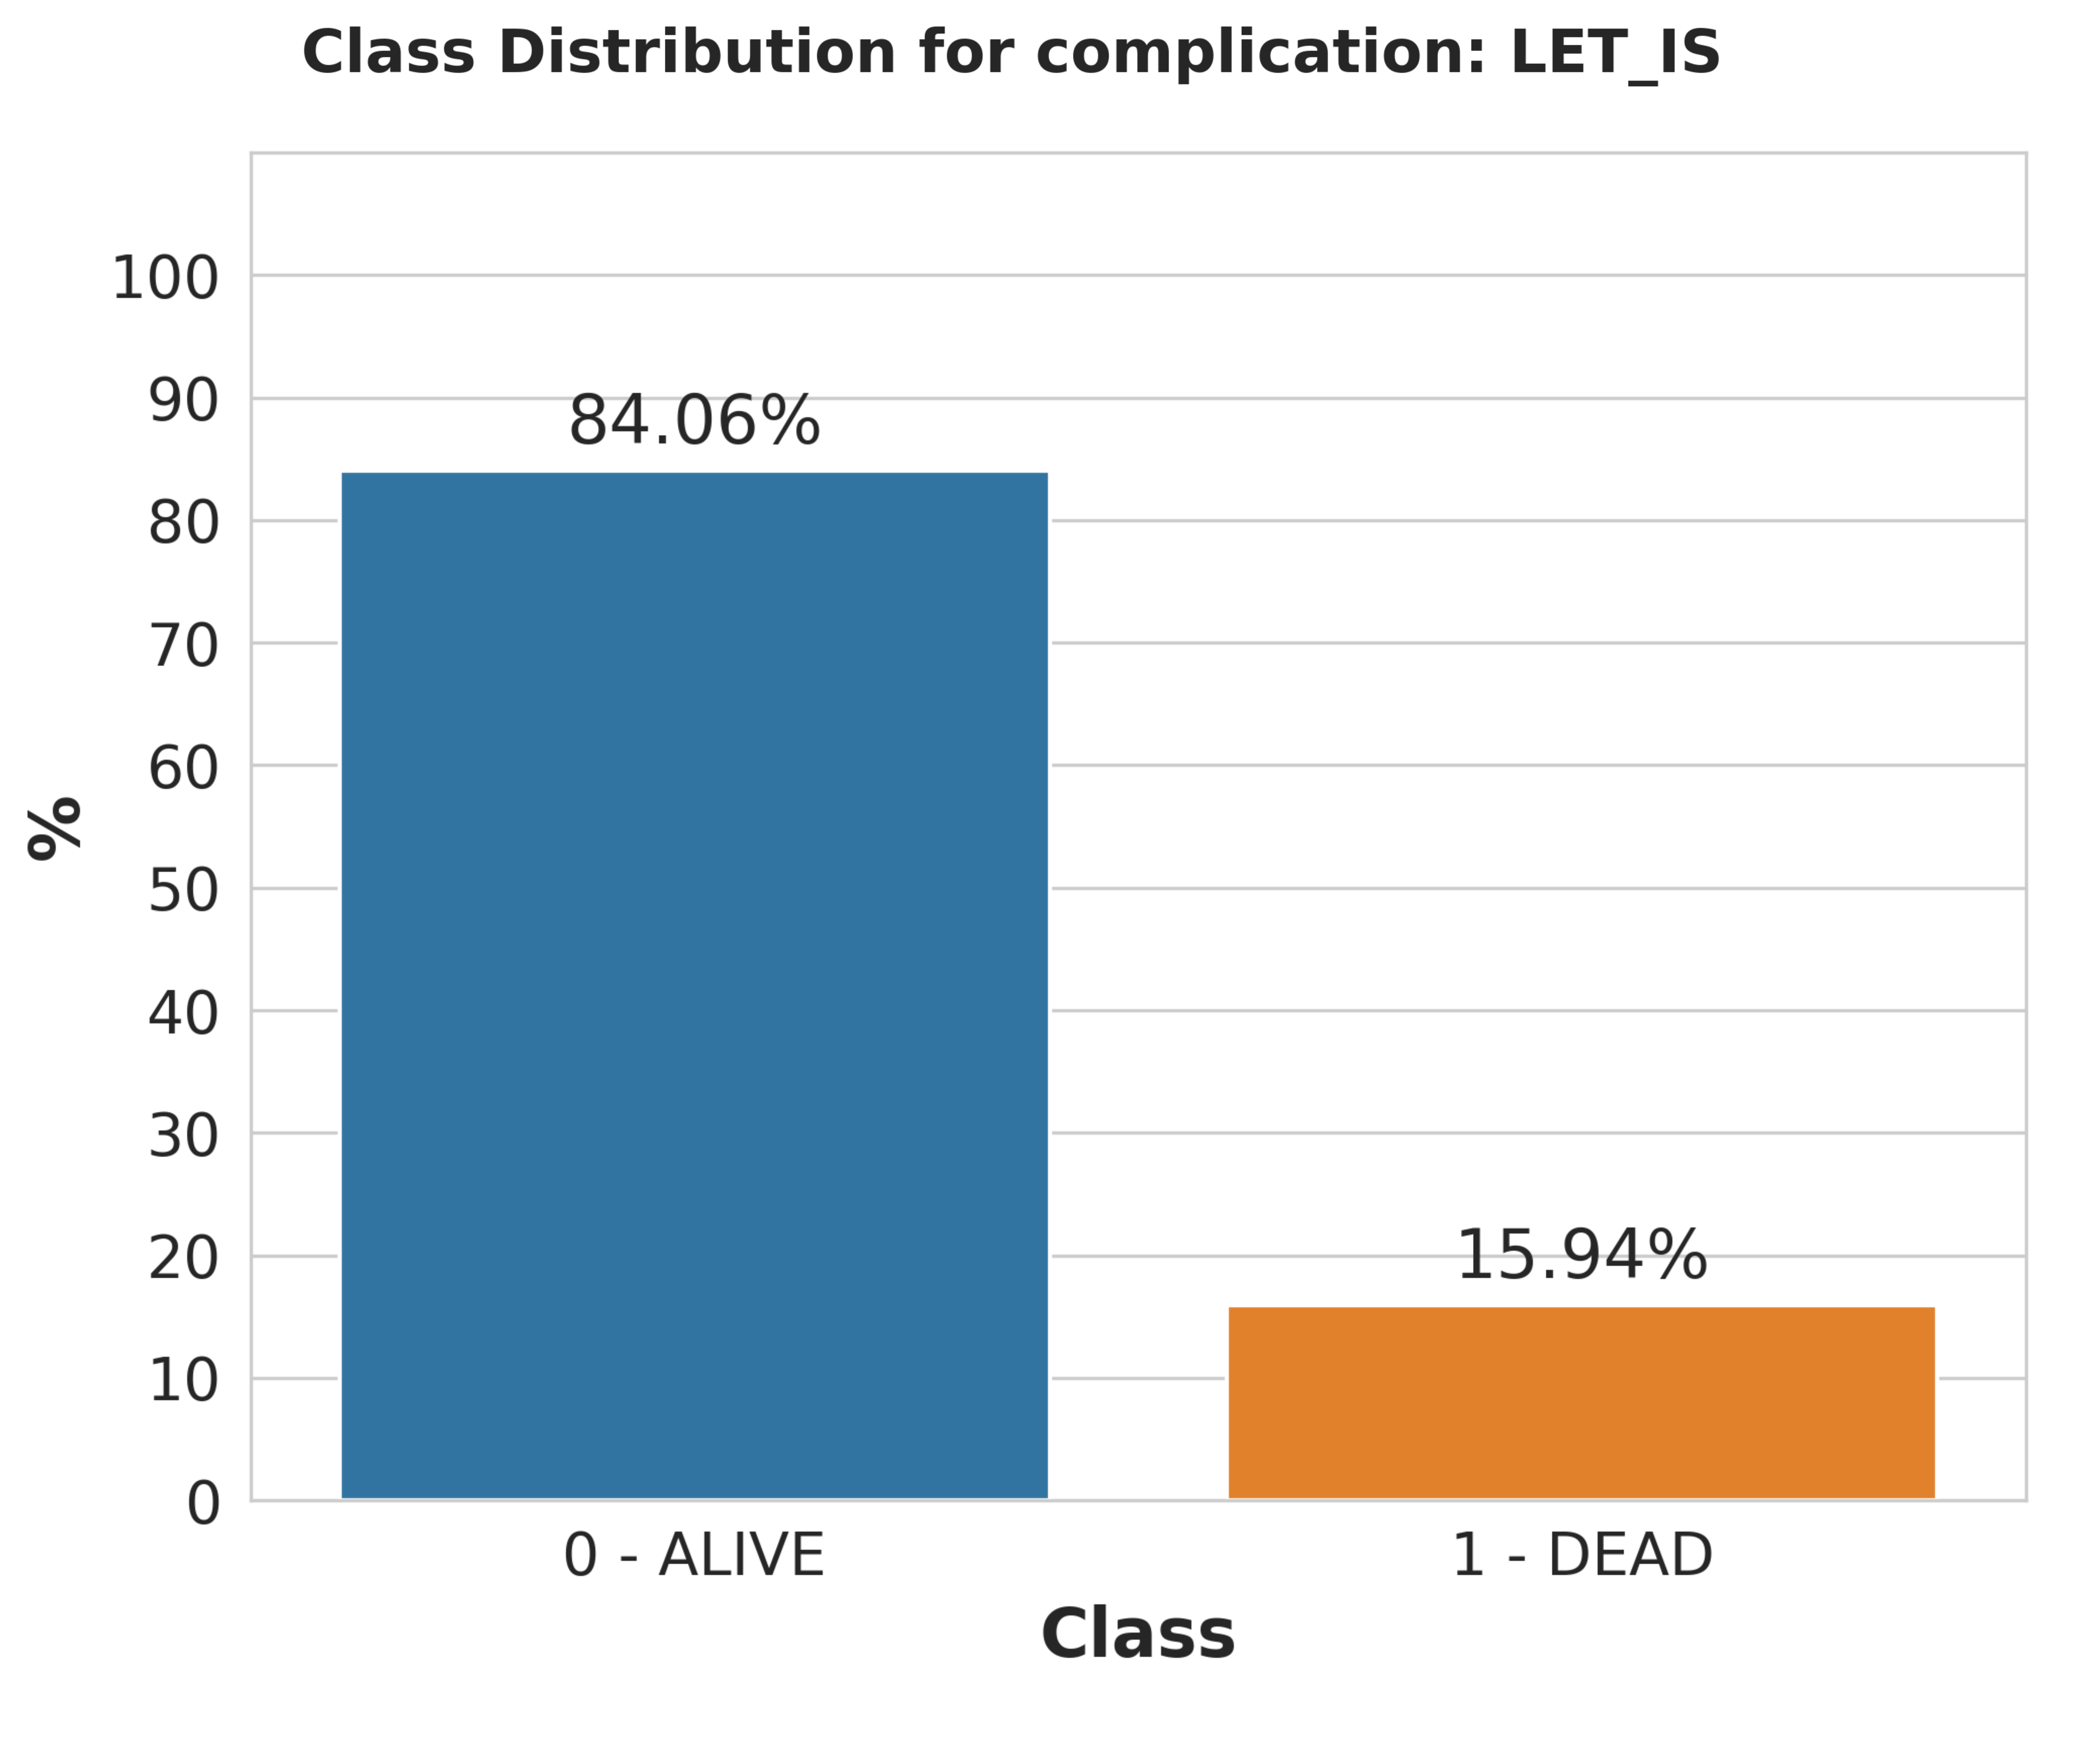
\includegraphics[width=\linewidth]{figures/Class_imbalance.png}
    \caption{Distribution of the target variable \texttt{LET\_IS}.}
    \label{fig:let_is-dist}
\end{figure}

The remaining features (\texttt{ID} excluded) were processed through a type-specific pipeline. Missing values were imputed using the median for numeric features and the mode for categorical features. Right-skewed numerical variables were transformed with log1p to mitigate skewness before standardization, whereas approximately normal numerical features were directly standardized using \texttt{StandardScaler}. Categorical features were encoded based on their semantics using \texttt{OneHotEncoder} (nominal), \texttt{LabelEncoder} (binary), and \texttt{OrdinalEncoder} (ordinal). The partially ordered feature \texttt{ZSN\_A} was transformed into two derived features (\texttt{HF\_right\_line}, \texttt{HF\_left\_line}) via a custom mapping to preserve its bidimensional severity structure.

Finally, feature selection was performed using \texttt{SelectKBest} with mutual information as the scoring criterion, treating the number of retained features ($k$) as a tunable hyperparameter. Crucially, to prevent data leakage, all imputation, transformation, and feature selection steps were strictly embedded within the cross-validation pipeline and fitted exclusively on the training folds.

\subsection{Imbalance-Aware and Cost-Sensitive Strategies}
Standard learning algorithms tend to favor the majority class, which is detrimental in mortality prediction where misclassifying a lethal outcome (false negative) carries severe clinical consequences \cite{Araf2024}. To address this, we implemented complementary strategies to mitigate imbalance at both the learning and decision levels.

\subsubsection{Learning-Level Strategies for Imbalanced Classification}

At the learning level, we considered three complementary strategies to address class imbalance.

\begin{itemize}
    \item \textbf{Data-level strategy (SMOTE):}  
    We adopted the Synthetic Minority Oversampling Technique (SMOTE) to increase the representation of the minority class in the training data.

    \item \textbf{Algorithm-level strategy (class-frequency-based weighting):}  
    For models supporting internal weighting mechanisms, class imbalance was handled through class-frequency-based weighting schemes (e.g., \texttt{class\_weight="balanced"} or \texttt{scale\_pos\_weight})

    \item \textbf{Cost-sensitive learning strategy:}  
   We implemented a cost-sensitive learning setting in which the training is explicitly guides by the asymmetric cost matrix detailed in Table~\ref{tab:cost-matrix}. Unlike frequency-based weighting, this strategy directly penalizes false negatives (FN = 10) ten times more heavily than false positives (FP = 1), reflecting their true clinical disparity.
   
\end{itemize}

\begin{table}[h]
    \centering
    \caption{Cost matrix adopted for cost-sensitive learning and decision-making.}
    \label{tab:cost-matrix}
    \begin{threeparttable}
        \begin{tabular}{clcc}
            \toprule
            & & \multicolumn{2}{c}{\textbf{Predicted Class}} \\
            \cmidrule(lr){3-4}
            & & \textbf{ALIVE (0)} & \textbf{DEAD (1)} \\
            \midrule
            \multirow{2}{*}{{\textbf{Actual Class}}} 
            & \textbf{ALIVE (0)} & TN = 0 & FP = 1 \\
            & \textbf{DEAD (1)}  & FN = 10 & TP = 0 \\
            \bottomrule
        \end{tabular}
    \end{threeparttable}
\end{table}

\subsubsection{Decision-Level Cost-Sensitive Prediction}

At the decision level, we compared the standard default probability threshold (0.5) against a post-hoc \textit{Minimum Expected Cost} (MEC) decision rule \cite{elkan2001}. Let \(P(y=k \mid x)\) denote the predicted posterior probability for class \(k\) given input \(x\), and let \(C_{k,c}\) denote the cost of predicting class \(c\) when the true class is \(k\). The MEC rule selects the class \(\hat{y}\)that minimizes the expected misclassification cost: 

\[
\hat{y} = \arg\min_{c} \sum_{k} P(y=k \mid x)\, C_{k,c}
\]

While SMOTE and sample weighting modify the underlying training objective, MEC acts strictly as a post-hoc decision mechanism applied to model outputs, forcing predictions into a regime aligned with the asymmetric costs in Table~\ref{tab:cost-matrix}.

\subsection{Predictive Models}
To evaluate predictive performance, we compared models ranging from a simple linear baseline to complex static and dynamic ensembles. The hyperparameter search spaces for all configurations are detailed in Table~\ref{tab:model-search-space}.

\subsubsection{Baseline Non-Ensemble Model}

As a probabilistic baseline, we implemented a \textbf{LogisticRegression} model with fixed configurations \texttt{solver="liblinear"}, \texttt{penalty="l2"}, and \texttt{max\_iter=1000}.

\subsubsection{Static Ensemble Models}
We considered four static ensembles representing different aggregation paradigms. 

For homogeneous tree-based ensembles, we implemented a bagging-based \textbf{RandomForestClassifier} (\texttt{criterion="gini"}, \texttt{bootstrap=True}) and a boosting-based \textbf{XGBClassifier} (\texttt{objective="binary:logistic"}, \texttt{eval\_metric="logloss"}). 

For heterogeneous aggregation, we implemented a \textbf{VotingClassifier} (uniform weights, soft voting) and a \textbf{StackingClassifier} (combining cross-validated predictions via Logistic Regression meta-estimator with \texttt{cv=3}). Both heterogeneous ensembles combined RandomForestClassifier, XGBClassifier, and an SGDClassifier as base learners. Importantly, these constituent learners were re-instantiated and independently optimized within the meta-ensemble pipelines to maximize predictive diversity.

\subsubsection{Dynamic Ensemble Selection}

Unlike static methods, DES tailors the active classifier subset for each specific query instance based on a local region of competence \cite{CRUZ2018195}. Operating on a base classifier pool generated by a BaggingClassifier of decision trees, we evaluated three distinct DES paradigms. To ensure comparability, competence estimation was performed on a dedicated dynamic selection dataset (DSEL), with all models sharing a neighborhood size of \texttt{k=8}, an instance hardness threshold of \texttt{IH\_rate=0.3}, and soft voting aggregation. Beyond these shared settings, we explored: (1) \textbf{KNORAE}, an oracle-based method which identifies local experts that perfectly classify the query's nearest neighbors, dynamically shrinking the region if no perfect oracle is initially found; (2) \textbf{DESKL}, a probabilistic method, which evaluates competence over the entire DSEL using a distance-weighted Gaussian potential function, selecting classifiers based on the Kullback--Leibler divergence of their output profiles; and (3) \textbf{METADES}, a meta-learning approach, which extracts local meta-features to train a secondary meta-classifier (implemented as a Multinomial Naive Bayes model) that explicitly predicts the competence of each base learner. Minor model-specific behaviors, such as dynamic frienemy pruning, were configured following standard literature defaults.

\begin{table*}[t]
\centering
\caption{Hyperparameter search spaces for the selected models.}\label{tab:model-search-space}
\begin{threeparttable}
\begin{tabular}{p{3cm} p{14.2cm}}

\toprule
\textbf{Model} & \textbf{Hyperparameter search space} \\

\midrule
\texttt{LogisticRegression} &
\texttt{C} \(\in [10^{-4}, 10^{4})\) (log-uniform); \texttt{tol} \(\in [10^{-5}, 10^{-2})\) (log-uniform); \texttt{fit\_intercept} \(\in \{\texttt{True}, \texttt{False}\}\) \\
\midrule

\texttt{SGDClassifier} &
\texttt{alpha} \(\in [10^{-5}, 10)\) (log-uniform); \texttt{penalty} \(\in \{\texttt{l2}, \texttt{l1}, \texttt{elasticnet}\}\); \texttt{l1\_ratio} \(\in [0, 1)\) \\
\midrule

\texttt{BaggingClassifier} (with \texttt{DecisionTree}) &
\texttt{n\_estimators} \(\in [100, 1000)\); \texttt{max\_samples} \(\in [0.5, 0.9)\);
\texttt{max\_depth} \(\in [3, 20)\); \texttt{min\_samples\_split} \(\in [2, 10)\); \texttt{min\_samples\_leaf} \(\in [1, 10)\);  \texttt{max\_leaf\_nodes} \(\in [2, 20)\); \texttt{min\_impurity\_decrease} \(\in [0.0, 0.1)\); \texttt{ccp\_alpha} \(\in [0.0, 0.01)\) \\
\midrule

\texttt{RandomForestClassifier} &
\texttt{n\_estimators} \(\in [100, 1000)\); \texttt{max\_samples} \(\in [0.5, 0.9)\); 
\texttt{max\_features} \(\in \{\texttt{sqrt}, \texttt{log2}, \texttt{None}\}\);
\texttt{max\_depth} \(\in [3, 20)\); \texttt{min\_samples\_split} \(\in [2, 10)\); \texttt{min\_samples\_leaf} \(\in [1, 10)\);  \texttt{max\_leaf\_nodes} \(\in [2, 20)\); \texttt{min\_impurity\_decrease} \(\in [0.0, 0.1)\); \texttt{ccp\_alpha} \(\in [0.0, 0.01)\) \\
\midrule

\texttt{XGBClassifier} &
\texttt{n\_estimators} \(\in [200, 800)\); \texttt{learning\_rate} \(\in [10^{-2}, 0.2)\) (log-uniform); \texttt{max\_depth} \(\in [3, 10)\); \texttt{subsample} \(\in [0.6, 1.0)\); \texttt{colsample\_bytree} \(\in [0.6, 1.0)\); \texttt{gamma} \(\in [0.0, 5.0)\); \texttt{reg\_alpha} \(\in [10^{-4}, 10)\) (log-uniform); \texttt{reg\_lambda} \(\in [10^{-4}, 10)\) (log-uniform); \texttt{min\_child\_weight} \(\in [1, 10)\) \\

\bottomrule
\end{tabular}
\end{threeparttable}
\end{table*}

\subsection{Learning Pipeline and Evaluation Protocol}
To obtain robust performance estimates while preserving class distributions, we evaluated all models using a repeated stratified 10 $\times$ 10 cross-validation protocol. Hyperparameter optimization was performed via nested stratified 5-fold cross-validation, employing a randomized search over 30 candidate configurations (\texttt{RandomizedSearchCV}). For the baseline and static ensembles, the optimal configuration was re-fitted on the entire outer training set and evaluated on the held-out test fold. For Dynamic Ensemble Selection (DES) methods, the evaluation protocol required an additional data partition to support dynamic selection. Specifically, the outer training folds were split into two subsets: 75\% of the data constituted the effective training set to learn and tune the base classifier pool, while the remaining 25\% served as the dynamic selection dataset (DSEL) to fit the competence estimation mechanism. The fully specified DES model was then evaluated on the outer test fold. Crucially, to prevent data leakage, all preprocessing operations—including imputation, feature transformation, feature selection, and optional SMOTE oversampling—were strictly embedded within the cross-validation pipelines. Consequently, these steps were fitted exclusively on the effective training data of each split and subsequently applied to the validation, DSEL, and test partitions without accessing future information.

\section{Experiment Setup} \label{sec:experiment-setup}
\subsection{Experimental Settings}

We defined seven experimental settings to systematically compare cost-insensitive, imbalance-aware, and cost-sensitive configurations under a common evaluation protocol. These configurations included a standard baseline (no resampling, no class weighting, and a default 0.5 decision threshold) and six imbalance-aware variants. The variants were formed by crossing three learning-level strategies—class-frequency-based weighting, cost-matrix-driven weighting ($\{0:1, 1:10\}$), and data-level oversampling (SMOTE) with two decision-level prediction rules: the standard 0.5 probability threshold and the Minimum Expected Cost (MEC) policy. For all MEC-based evaluations, the decision rule utilized the asymmetric cost matrix defined in Section~\ref{sec:methodology}.

\subsection{Evaluation Metrics}
For each cross-validation fold, we assessed general discriminative performance using standard classification metrics: Accuracy, Precision, Recall, F1-score, and ROC-AUC. However, the primary criterion for overall model comparison was a domain-specific \textbf{Average Cost per Prediction} (AvgCost), defined as \(\text{AvgCost} = (1 \cdot \text{FP} + 10 \cdot \text{FN}) / \text{N}\), where \(\text{FP}\) and \(\text{FN}\)denote the numbers of false positives and false negatives, respectively, and \(\text{N}\) is the total number of predictions. Lower AvgCost values indicate better cost-sensitive performance. Finally, to assess whether the observed differences in AvgCost between model configurations were statistically significant, we applied the corrected resampled t-test with a standard significance level of $\alpha = 0.05$.

\subsection{Implementation Details}

Experiments were implemented in Python 3.10, using scikit-learn 1.6.1, imbalanced-learn 0.14.0, and DESlib 0.3.7. The experiments were executed on a Lenovo ThinkPad T14 Gen 4 equipped with an Intel Core i7-1355U processor, 16\,GB of DDR5 RAM, and a 512\,GB PCIe Gen4 SSD. The full implementation is publicly available in the following GitHub repository: \url{https://github.com/LeonardoSaccotelli/Cost-Sensitive-Learning-For-Myocardial-Infarction-Mortality-Prediction}. 

\section{Results} \label{sec:results}
\subsection{Overall Performance and Learning-Level Impact}Table~\ref{tab:summary} reports the performance of all model variants, sorted by Average Cost. Explicitly addressing class imbalance substantially improved performance across all model families compared to their cost-insensitive baselines. The best overall configuration was StackingClassifier with cost-sensitive learning and the standard decision rule (AvgCost: $0.5024 \pm 0.1150$), followed closely by StackingClassifier with SMOTE and MEC ($0.5316 \pm 0.0995$) and XGBClassifier with cost-sensitive learning ($0.5367 \pm 0.1283$). Among learning-level strategies, cost-sensitive learning driven by asymmetric weights $\{0:1, 1:10\}$ was overwhelmingly the most effective, producing the top configurations for StackingClassifier, XGBClassifier, RandomForestClassifier, LogisticRegression, and the DESKL method. While balanced frequency weighting improved upon baselines, it generally underperformed the cost-matrix-driven alternative. Notably, standard metrics alone failed to capture the task's asymmetric clinical objective: the baseline StackingClassifier achieved the highest overall Accuracy ($0.8809 \pm 0.0180$), but ranked poorly in AvgCost ($0.9830 \pm 0.1369$), confirming Average Cost as the necessary criterion for model evaluation.

\subsection{Effect of the MEC Decision Rule}
Comparing the standard threshold with the MEC decision rule reveals a severe shift in the models' operating points. MEC consistently pushed recall toward its maximum (often reaching $1.0000$) at the cost of drastically lower precision and accuracy. This caused numerous MEC configurations to converge to near-identical operating behaviors, plateauing around an Average Cost of $0.84$. Consequently, MEC was not uniformly beneficial. For models already utilizing cost-sensitive or balanced training weights, applying MEC often degraded AvgCost compared to the standard rule. However, MEC proved highly effective when paired with purely data-level interventions like SMOTE, drastically improving the StackingClassifier (AvgCost dropping from $0.7614$ to $0.5316$) and XGBClassifier (from $0.9167$ to $0.5911$). Thus, MEC acts as a complementary decision mechanism whose efficacy depends heavily on the underlying training strategy.

\subsection{Static Ensembles versus DES}
Static ensembles dominated the top of the ranking, with StackingClassifier and XGBClassifier achieving the lowest Average Costs. Among the dynamic ensemble selection methods, DESKL with cost-sensitive learning and the standard rule yielded the strongest result ($0.5872 \pm 0.1317$). While competitive with several static models, it did not surpass the best stacking and boosting architectures. METADES achieved reasonable results, whereas KNORAE remained generally uncompetitive (AvgCost $> 0.83$). Overall, dynamic selection provided robust cost-sensitive performance but did not systematically outperform fixed static ensembles.

\begin{table*}[h]
    \centering
    \caption{Performance metrics across all models and experiment settings, sorted by ascending Average Cost.}
    \label{tab:summary}
    \begin{threeparttable}
        \resizebox{\textwidth}{!}{
        \begin{tabular}{lcc|cccccc}
            \toprule
            \textbf{Model} & \textbf{Imbalance Strategy} & \textbf{Threshold} & \textbf{Average Cost} & \textbf{ROC\_AUC} & \textbf{Accuracy} & \textbf{Precision} & \textbf{Recall} & \textbf{F1} \\
            \midrule
            StackingClassifier & Cost-sensitive & Standard & \textbf{0.5024 $\pm$ 0.1150} & \textbf{0.8697 $\pm$ 0.0389} & 0.7271 $\pm$ 0.0506 & 0.3570 $\pm$ 0.0477 & 0.8402 $\pm$ 0.0711 & 0.4990 $\pm$ 0.0515 \\
            StackingClassifier & SMOTE & MEC & 0.5316 $\pm$ 0.0995 & 0.8615 $\pm$ 0.0412 & 0.6104 $\pm$ 0.0768 & 0.2845 $\pm$ 0.0444 & 0.9012 $\pm$ 0.0721 & 0.4297 $\pm$ 0.0466 \\
            XGBClassifier & Cost-sensitive & Standard & 0.5367 $\pm$ 0.1283 & 0.8631 $\pm$ 0.0361 & 0.7587 $\pm$ 0.0529 & 0.3878 $\pm$ 0.0606 & 0.7945 $\pm$ 0.0907 & 0.5165 $\pm$ 0.0561 \\
            StackingClassifier & Balanced & Standard & 0.5510 $\pm$ 0.1380 & 0.8689 $\pm$ 0.0375 & 0.7971 $\pm$ 0.0348 & 0.4285 $\pm$ 0.0551 & 0.7577 $\pm$ 0.0861 & 0.5453 $\pm$ 0.0579 \\
            RandomForestClassifier & Cost-sensitive & Standard & 0.5562 $\pm$ 0.1069 & 0.8424 $\pm$ 0.0413 & 0.5377 $\pm$ 0.1172 & 0.2569 $\pm$ 0.0438 & 0.9347 $\pm$ 0.0609 & 0.4002 $\pm$ 0.0526 \\
            LogisticRegression & Cost-sensitive & Standard & 0.5596 $\pm$ 0.1382 & 0.8372 $\pm$ 0.0449 & 0.6781 $\pm$ 0.0477 & 0.3136 $\pm$ 0.0398 & 0.8346 $\pm$ 0.0825 & 0.4548 $\pm$ 0.0495 \\
            DESKL & Cost-sensitive & Standard & 0.5872 $\pm$ 0.1317 & 0.8268 $\pm$ 0.0470 & 0.6527 $\pm$ 0.0746 & 0.3004 $\pm$ 0.0485 & 0.8332 $\pm$ 0.0853 & 0.4387 $\pm$ 0.0541 \\
            XGBClassifier & SMOTE & MEC & 0.5911 $\pm$ 0.1410 & 0.8334 $\pm$ 0.0581 & 0.5469 $\pm$ 0.1963 & 0.2768 $\pm$ 0.0837 & 0.9041 $\pm$ 0.0855 & 0.4138 $\pm$ 0.0911 \\
            XGBClassifier & Balanced & Standard & 0.5968 $\pm$ 0.1459 & 0.8688 $\pm$ 0.0363 & 0.8309 $\pm$ 0.0272 & 0.4833 $\pm$ 0.0560 & 0.7023 $\pm$ 0.0934 & \textbf{0.5699 $\pm$ 0.0598} \\
            XGBClassifier & Balanced & MEC & 0.5979 $\pm$ 0.0984 & 0.8682 $\pm$ 0.0355 & 0.4444 $\pm$ 0.1086 & 0.2244 $\pm$ 0.0316 & 0.9706 $\pm$ 0.0417 & 0.3631 $\pm$ 0.0410 \\
            LogisticRegression & Balanced & Standard & 0.6206 $\pm$ 0.1527 & 0.8367 $\pm$ 0.0446 & 0.7687 $\pm$ 0.0350 & 0.3851 $\pm$ 0.0498 & 0.7290 $\pm$ 0.0949 & 0.5023 $\pm$ 0.0585 \\
            LogisticRegression & SMOTE & Standard & 0.6229 $\pm$ 0.1316 & 0.8330 $\pm$ 0.0465 & 0.7648 $\pm$ 0.0381 & 0.3818 $\pm$ 0.0486 & 0.7302 $\pm$ 0.0834 & 0.4993 $\pm$ 0.0525 \\
            VotingClassifier & Cost-sensitive & Standard & 0.6286 $\pm$ 0.1549 & 0.8386 $\pm$ 0.0472 & 0.5637 $\pm$ 0.1763 & 0.2720 $\pm$ 0.0690 & 0.8662 $\pm$ 0.0905 & 0.4068 $\pm$ 0.0785 \\
            METADES & Cost-sensitive & Standard & 0.6352 $\pm$ 0.1432 & 0.8273 $\pm$ 0.0506 & 0.7317 $\pm$ 0.0611 & 0.3526 $\pm$ 0.0588 & 0.7446 $\pm$ 0.1010 & 0.4740 $\pm$ 0.0580 \\
            VotingClassifier & Balanced & Standard & 0.6441 $\pm$ 0.1550 & 0.8533 $\pm$ 0.0418 & 0.7727 $\pm$ 0.0826 & 0.4121 $\pm$ 0.0948 & 0.7097 $\pm$ 0.1192 & 0.5088 $\pm$ 0.0744 \\
            XGBClassifier & Cost-sensitive & MEC & 0.6946 $\pm$ 0.1088 & 0.8639 $\pm$ 0.0380 & 0.3294 $\pm$ 0.1250 & 0.1947 $\pm$ 0.0289 & 0.9833 $\pm$ 0.0340 & 0.3239 $\pm$ 0.0390 \\
            RandomForestClassifier & Balanced & Standard & 0.7086 $\pm$ 0.1392 & 0.8417 $\pm$ 0.0401 & 0.8033 $\pm$ 0.0341 & 0.4287 $\pm$ 0.0645 & 0.6438 $\pm$ 0.0838 & 0.5125 $\pm$ 0.0649 \\
            LogisticRegression & SMOTE & MEC & 0.7164 $\pm$ 0.0726 & 0.8322 $\pm$ 0.0466 & 0.3042 $\pm$ 0.0837 & 0.1868 $\pm$ 0.0184 & 0.9857 $\pm$ 0.0269 & 0.3135 $\pm$ 0.0251 \\
            LogisticRegression & Balanced & MEC & 0.7282 $\pm$ 0.0691 & 0.8367 $\pm$ 0.0448 & 0.2901 $\pm$ 0.0724 & 0.1834 $\pm$ 0.0150 & 0.9873 $\pm$ 0.0265 & 0.3089 $\pm$ 0.0211 \\
            VotingClassifier & SMOTE & Standard & 0.7462 $\pm$ 0.2047 & 0.8420 $\pm$ 0.0414 & 0.7649 $\pm$ 0.0922 & 0.4080 $\pm$ 0.1109 & 0.6443 $\pm$ 0.1733 & 0.4729 $\pm$ 0.0758 \\
            LogisticRegression & Cost-sensitive & MEC & 0.7610 $\pm$ 0.0539 & 0.8382 $\pm$ 0.0463 & 0.2516 $\pm$ 0.0577 & 0.1755 $\pm$ 0.0109 & 0.9912 $\pm$ 0.0245 & 0.2980 $\pm$ 0.0155 \\
            StackingClassifier & SMOTE & Standard & 0.7614 $\pm$ 0.1683 & 0.8639 $\pm$ 0.0383 & 0.8615 $\pm$ 0.0259 & 0.5746 $\pm$ 0.0838 & 0.5665 $\pm$ 0.1098 & 0.5641 $\pm$ 0.0770 \\
            DESKL & Balanced & Standard & 0.7861 $\pm$ 0.1423 & 0.8309 $\pm$ 0.0440 & 0.8265 $\pm$ 0.0341 & 0.4736 $\pm$ 0.0828 & 0.5737 $\pm$ 0.0874 & 0.5150 $\pm$ 0.0723 \\
            VotingClassifier & SMOTE & MEC & 0.8243 $\pm$ 0.0419 & 0.8443 $\pm$ 0.0410 & 0.1780 $\pm$ 0.0447 & 0.1628 $\pm$ 0.0083 & 0.9984 $\pm$ 0.0078 & 0.2799 $\pm$ 0.0119 \\
            StackingClassifier & Balanced & MEC & 0.8349 $\pm$ 0.0251 & 0.8686 $\pm$ 0.0340 & 0.1651 $\pm$ 0.0251 & 0.1607 $\pm$ 0.0050 & \textbf{1.0000 $\pm$ 0.0000} & 0.2768 $\pm$ 0.0072 \\
            VotingClassifier & Balanced & MEC & 0.8354 $\pm$ 0.0181 & 0.8567 $\pm$ 0.0440 & 0.1669 $\pm$ 0.0276 & 0.1608 $\pm$ 0.0046 & 0.9984 $\pm$ 0.0097 & 0.2769 $\pm$ 0.0064 \\
            KNORAE & Balanced & MEC & 0.8375 $\pm$ 0.0337 & 0.7250 $\pm$ 0.0531 & 0.1723 $\pm$ 0.0134 & 0.1610 $\pm$ 0.0036 & 0.9932 $\pm$ 0.0221 & 0.2770 $\pm$ 0.0059 \\
            VotingClassifier & Cost-sensitive & MEC & 0.8389 $\pm$ 0.0072 & 0.8421 $\pm$ 0.0461 & 0.1611 $\pm$ 0.0072 & 0.1599 $\pm$ 0.0022 & \textbf{1.0000 $\pm$ 0.0000} & 0.2757 $\pm$ 0.0032 \\
            KNORAE & Cost-sensitive & MEC & 0.8398 $\pm$ 0.0472 & 0.7405 $\pm$ 0.0538 & 0.1894 $\pm$ 0.0265 & 0.1624 $\pm$ 0.0057 & 0.9797 $\pm$ 0.0280 & 0.2786 $\pm$ 0.0089 \\
            METADES & SMOTE & MEC & 0.8400 $\pm$ 0.0025 & 0.7399 $\pm$ 0.0638 & 0.1600 $\pm$ 0.0025 & 0.1597 $\pm$ 0.0017 & \textbf{1.0000 $\pm$ 0.0000} & 0.2755 $\pm$ 0.0025 \\
            METADES & Balanced & MEC & 0.8403 $\pm$ 0.0017 & 0.8186 $\pm$ 0.0440 & 0.1597 $\pm$ 0.0017 & 0.1597 $\pm$ 0.0017 & \textbf{1.0000 $\pm$ 0.0000} & 0.2754 $\pm$ 0.0025 \\
            METADES & Cost-sensitive & MEC & 0.8403 $\pm$ 0.0017 & 0.8281 $\pm$ 0.0433 & 0.1597 $\pm$ 0.0017 & 0.1597 $\pm$ 0.0017 & \textbf{1.0000 $\pm$ 0.0000} & 0.2754 $\pm$ 0.0025 \\
            DESKL & Balanced & MEC & 0.8403 $\pm$ 0.0017 & 0.8290 $\pm$ 0.0434 & 0.1597 $\pm$ 0.0017 & 0.1597 $\pm$ 0.0017 & \textbf{1.0000 $\pm$ 0.0000} & 0.2754 $\pm$ 0.0025 \\
            DESKL & Cost-sensitive & MEC & 0.8403 $\pm$ 0.0017 & 0.8270 $\pm$ 0.0436 & 0.1597 $\pm$ 0.0017 & 0.1597 $\pm$ 0.0017 & \textbf{1.0000 $\pm$ 0.0000} & 0.2754 $\pm$ 0.0025 \\
            DESKL & SMOTE & MEC & 0.8403 $\pm$ 0.0017 & 0.7888 $\pm$ 0.0477 & 0.1597 $\pm$ 0.0017 & 0.1597 $\pm$ 0.0017 & \textbf{1.0000 $\pm$ 0.0000} & 0.2754 $\pm$ 0.0025 \\
            RandomForestClassifier & Balanced & MEC & 0.8403 $\pm$ 0.0017 & 0.8448 $\pm$ 0.0402 & 0.1597 $\pm$ 0.0017 & 0.1597 $\pm$ 0.0017 & \textbf{1.0000 $\pm$ 0.0000} & 0.2754 $\pm$ 0.0025 \\
            RandomForestClassifier & Cost-sensitive & MEC & 0.8403 $\pm$ 0.0017 & 0.8431 $\pm$ 0.0423 & 0.1597 $\pm$ 0.0017 & 0.1597 $\pm$ 0.0017 & \textbf{1.0000 $\pm$ 0.0000} & 0.2754 $\pm$ 0.0025 \\
            RandomForestClassifier & SMOTE & MEC & 0.8403 $\pm$ 0.0017 & 0.7908 $\pm$ 0.0492 & 0.1597 $\pm$ 0.0017 & 0.1597 $\pm$ 0.0017 & \textbf{1.0000 $\pm$ 0.0000} & 0.2754 $\pm$ 0.0025 \\
            StackingClassifier & Cost-sensitive & MEC & 0.8403 $\pm$ 0.0017 & 0.8687 $\pm$ 0.0370 & 0.1597 $\pm$ 0.0017 & 0.1597 $\pm$ 0.0017 & \textbf{1.0000 $\pm$ 0.0000} & 0.2754 $\pm$ 0.0025 \\
            KNORAE & SMOTE & MEC & 0.8422 $\pm$ 0.0240 & 0.7013 $\pm$ 0.0616 & 0.1664 $\pm$ 0.0172 & 0.1601 $\pm$ 0.0033 & 0.9940 $\pm$ 0.0174 & 0.2758 $\pm$ 0.0050 \\
            RandomForestClassifier & SMOTE & Standard & 0.8492 $\pm$ 0.1704 & 0.7908 $\pm$ 0.0549 & 0.7944 $\pm$ 0.0470 & 0.4050 $\pm$ 0.0853 & 0.5520 $\pm$ 0.1220 & 0.4604 $\pm$ 0.0829 \\
            KNORAE & Cost-sensitive & Standard & 0.8515 $\pm$ 0.1659 & 0.7396 $\pm$ 0.0583 & 0.7382 $\pm$ 0.0397 & 0.3272 $\pm$ 0.0536 & 0.5894 $\pm$ 0.1083 & 0.4180 $\pm$ 0.0646 \\
            DESKL & SMOTE & Standard & 0.8944 $\pm$ 0.1466 & 0.7908 $\pm$ 0.0485 & 0.8155 $\pm$ 0.0423 & 0.4516 $\pm$ 0.1007 & 0.5058 $\pm$ 0.0962 & 0.4692 $\pm$ 0.0770 \\
            METADES & Balanced & Standard & 0.8975 $\pm$ 0.1689 & 0.8199 $\pm$ 0.0463 & 0.8348 $\pm$ 0.0265 & 0.4854 $\pm$ 0.0857 & 0.4902 $\pm$ 0.1070 & 0.4839 $\pm$ 0.0876 \\
            KNORAE & Balanced & Standard & 0.9104 $\pm$ 0.1678 & 0.7337 $\pm$ 0.0575 & 0.7652 $\pm$ 0.0318 & 0.3476 $\pm$ 0.0595 & 0.5297 $\pm$ 0.1056 & 0.4178 $\pm$ 0.0707 \\
            XGBClassifier & SMOTE & Standard & 0.9167 $\pm$ 0.1490 & 0.8322 $\pm$ 0.0565 & 0.8476 $\pm$ 0.0474 & 0.5669 $\pm$ 0.1458 & 0.4680 $\pm$ 0.0997 & 0.4992 $\pm$ 0.0914 \\
            XGBClassifier & None & Standard & 0.9484 $\pm$ 0.1368 & 0.8657 $\pm$ 0.0368 & 0.8766 $\pm$ 0.0185 & 0.6896 $\pm$ 0.1038 & 0.4259 $\pm$ 0.0860 & 0.5214 $\pm$ 0.0799 \\
            StackingClassifier & None & Standard & 0.9830 $\pm$ 0.1369 & 0.8693 $\pm$ 0.0347 & \textbf{0.8809 $\pm$ 0.0180} & 0.7442 $\pm$ 0.1109 & 0.3988 $\pm$ 0.0864 & 0.5131 $\pm$ 0.0842 \\
            KNORAE & SMOTE & Standard & 0.9980 $\pm$ 0.1687 & 0.7037 $\pm$ 0.0562 & 0.7589 $\pm$ 0.0327 & 0.3264 $\pm$ 0.0633 & 0.4733 $\pm$ 0.1065 & 0.3840 $\pm$ 0.0736 \\
            METADES & SMOTE & Standard & 1.0012 $\pm$ 0.1561 & 0.7570 $\pm$ 0.0652 & 0.8157 $\pm$ 0.0297 & 0.4309 $\pm$ 0.0833 & 0.4315 $\pm$ 0.0978 & 0.4265 $\pm$ 0.0785 \\
            LogisticRegression & None & Standard & 1.0115 $\pm$ 0.1624 & 0.8241 $\pm$ 0.0639 & 0.8592 $\pm$ 0.0393 & 0.6126 $\pm$ 0.1310 & 0.3940 $\pm$ 0.1006 & 0.4720 $\pm$ 0.1015 \\
            VotingClassifier & None & Standard & 1.0925 $\pm$ 0.2184 & 0.8557 $\pm$ 0.0394 & 0.8682 $\pm$ 0.0187 & 0.7014 $\pm$ 0.1531 & 0.3314 $\pm$ 0.1433 & 0.4283 $\pm$ 0.1370 \\
            KNORAE & None & Standard & 1.2171 $\pm$ 0.1505 & 0.7166 $\pm$ 0.0654 & 0.8351 $\pm$ 0.0233 & 0.4766 $\pm$ 0.1649 & 0.2678 $\pm$ 0.0978 & 0.3340 $\pm$ 0.1061 \\
            METADES & None & Standard & 1.3920 $\pm$ 0.1403 & 0.7626 $\pm$ 0.0773 & 0.8486 $\pm$ 0.0146 & 0.6062 $\pm$ 0.2867 & 0.1366 $\pm$ 0.0911 & 0.2117 $\pm$ 0.1240 \\
            DESKL & None & Standard & 1.3997 $\pm$ 0.1115 & 0.7928 $\pm$ 0.0840 & 0.8569 $\pm$ 0.0113 & \textbf{0.8045 $\pm$ 0.2820} & 0.1255 $\pm$ 0.0696 & 0.2121 $\pm$ 0.1069 \\
            RandomForestClassifier & None & Standard & 1.4174 $\pm$ 0.1098 & 0.7890 $\pm$ 0.0809 & 0.8559 $\pm$ 0.0111 & 0.7944 $\pm$ 0.3280 & 0.1138 $\pm$ 0.0709 & 0.1938 $\pm$ 0.1124 \\
            \bottomrule
        \end{tabular}
        }
    \end{threeparttable}
\end{table*}


\subsection{Statistical Significance Analysis} 
To assess whether these observations were statistically meaningful, we applied the corrected resampled t-test ($\alpha = 0.05$). The pairwise significance heatmap (Figure~\ref{fig:heatmap-pvalue-all}) confirms that the observed ranking reflects substantial performance differences. The strongest statistical evidence emerged when comparing cost-sensitive configurations (with standard decision rules) against their respective baselines, confirming the significant benefit of imbalance-aware training. The top-ranked StackingClassifier and XGBClassifier models were significantly superior to a vast majority of alternative configurations, including baseline settings and weaker DES methods. Furthermore, the heatmap visually validates the convergence behavior of the MEC rule: large blocks of MEC-based configurations showed no statistically significant differences from one another. Finally, while DESKL proved significantly better than weaker baselines, the statistical analysis confirms it did not hold a systematic advantage over the top-tier static ensembles.

\begin{figure*}[h]
    \centering
    
\includegraphics[width=\textwidth]{figures/corrected_resampled_ttest_average_cost_heatmap.png}
\caption{Pairwise p-value heatmap of the corrected resampled t-test on AvgCost across all evaluated configurations.}
    \label{fig:heatmap-pvalue-all}
\end{figure*}

\section{Discussion and Conclusion} \label{sec:discussion-conclusion}

This study demonstrates that explicitly addressing class imbalance via cost-sensitive learning is crucial for admission-time myocardial infarction mortality prediction. Our systematic evaluation reveals that cost-sensitive learning combined with a standard decision threshold provides the most reliable overall performance. Static ensemble approaches, particularly StackingClassifier and XGBClassifier, proved to be the most robust architectures, ultimately outperforming the most competitive dynamic ensemble selection method (DESKL) in this specific context.

Despite these strong baselines, several limitations present clear avenues for future research. First, because the dataset originates from an older, relatively limited clinical cohort, validating this framework on contemporary, large-scale datasets is necessary to ensure modern clinical applicability. Second, our pipeline focuses exclusively on admission-time binary mortality; future work should extend this approach to predict specific causes of death, non-lethal complications, and dynamic risks at later hospitalization stages. Finally, while representative, the evaluated DES methods do not exhaust the dynamic selection literature. Exploring alternative pool-generation strategies alongside dedicated threshold calibration techniques could further optimize the critical trade-off between false positives and false negatives in intensive care settings.

\bibliographystyle{IEEEtran}
\bibliography{biblio}
\end{document}